%%%%%%%%%%%%%%%%%%%%%%%%%%%%%%%%%%%%%%%%%
% Beamer Presentation
% LaTeX Template
% Version 1.0 (10/11/12)
%
% This template has been downloaded from:
% http://www.LaTeXTemplates.com
%
% License:
% CC BY-NC-SA 3.0 (http://creativecommons.org/licenses/by-nc-sa/3.0/)
%
%%%%%%%%%%%%%%%%%%%%%%%%%%%%%%%%%%%%%%%%%

%----------------------------------------------------------------------------------------
%	PACKAGES AND THEMES
%----------------------------------------------------------------------------------------

\documentclass{beamer}

\mode<presentation> {

% The Beamer class comes with a number of default slide themes
% which change the colors and layouts of slides. Below this is a list
% of all the themes, uncomment each in turn to see what they look like.

%\usetheme{default}
%\usetheme{AnnArbor}
%\usetheme{Antibes}
%\usetheme{Bergen}
%\usetheme{Berkeley}
%\usetheme{Berlin}
%\usetheme{Boadilla}
%\usetheme{CambridgeUS}
%\usetheme{Copenhagen}
%\usetheme{Darmstadt}
%\usetheme{Dresden}
%\usetheme{Frankfurt}
%\usetheme{Goettingen}
%\usetheme{Hannover}
%\usetheme{Ilmenau}
%\usetheme{JuanLesPins}
%\usetheme{Luebeck}
\usetheme{Madrid}
%\usetheme{Malmoe}
%\usetheme{Marburg}
%\usetheme{Montpellier}
%\usetheme{PaloAlto}
%\usetheme{Pittsburgh}
%\usetheme{Rochester}
%\usetheme{Singapore}
%\usetheme{Szeged}
%\usetheme{Warsaw}

% As well as themes, the Beamer class has a number of color themes
% for any slide theme. Uncomment each of these in turn to see how it
% changes the colors of your current slide theme.

%\usecolortheme{albatross}
%\usecolortheme{beaver}
%\usecolortheme{beetle}
%\usecolortheme{crane}
%\usecolortheme{dolphin}
%\usecolortheme{dove}
%\usecolortheme{fly}
%\usecolortheme{lily}
%\usecolortheme{orchid}
%\usecolortheme{rose}
%\usecolortheme{seagull}
%\usecolortheme{seahorse}
%\usecolortheme{whale}
%\usecolortheme{wolverine}

%\setbeamertemplate{footline} % To remove the footer line in all slides uncomment this line
%\setbeamertemplate{footline}[page number] % To replace the footer line in all slides with a simple slide count uncomment this line

%\setbeamertemplate{navigation symbols}{} % To remove the navigation symbols from the bottom of all slides uncomment this line
}

\usepackage{graphicx} % Allows including images
\usepackage{booktabs} % Allows the use of \toprule, \midrule and \bottomrule in tables
\usepackage{listings}
\usepackage{amsmath}
\usepackage{algpseudocode,algorithm,algorithmicx}

\lstdefinestyle{customjava}{
  breaklines=true,
  frame=L,
  xleftmargin=\parindent,
  language=Java,
  showstringspaces=false,
  basicstyle=\footnotesize\ttfamily,
  keywordstyle=\bfseries\color{green!40!black},
  commentstyle=\itshape\color{gray!40!black},
  identifierstyle=\color{blue},
  stringstyle=\color{orange},
}

\lstdefinestyle{customcpp}{
  breaklines=true,
  frame=L,
  xleftmargin=\parindent,
  language=C++,
  showstringspaces=false,
  basicstyle=\footnotesize\ttfamily,
  keywordstyle=\bfseries\color{green!40!black},
  commentstyle=\itshape\color{gray!40!black},
  identifierstyle=\color{blue},
  stringstyle=\color{orange},
}
%----------------------------------------------------------------------------------------
%	TITLE PAGE
%----------------------------------------------------------------------------------------

\title[Practical Memory Management]{Practical Memory Management} % The short title appears at the bottom of every slide, the full title is only on the title page

\author{Jonathan Windle} % Your name
\institute[UEA] % Your institution as it will appear on the bottom of every slide, may be shorthand to save space
{
University of East Anglia \\ % Your institution for the title page
\medskip
\textit{J.Windle@uea.ac.uk} % Your email address
}
\date{\today} % Date, can be changed to a custom date

\begin{document}

\begin{frame}
\titlepage % Print the title page as the first slide
\end{frame}

\begin{frame}[allowframebreaks]
\frametitle{Overview} % Table of contents slide, comment this block out to remove it
\tableofcontents % Throughout your presentation, if you choose to use \section{} and \subsection{} commands, these will automatically be printed on this slide as an overview of your presentation
\end{frame}

%-------------------------------------------------------------------
\section{Memory Management Unit}
\begin{frame}
\frametitle{Memory Management Unit (MMU)}
\begin{itemize}
\item MMU is hardware that provides the translation from a virtual address to a physical address
\item Works in conjunction with OS memory manager that allocates/deallocates memory
\item MMU sits between CPU and system bus
\item MMU allows implementation of virtual/logical addresses
\item Location:\\
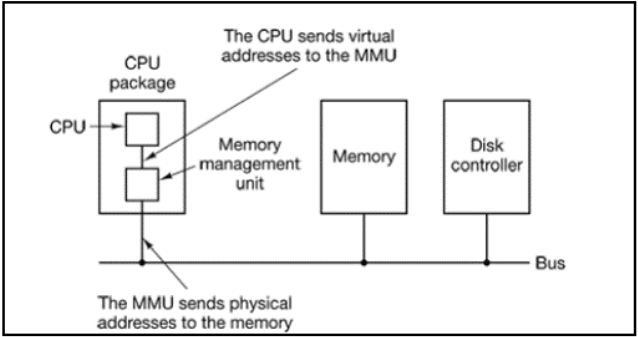
\includegraphics[scale=.3]{loc.png}
\end{itemize}
\end{frame}
%-----------------------------------------------------------------
\subsection{Provides}
\begin{frame}
\frametitle{Provides}
\begin{itemize}
\item Non-Contiguous memory segmentation by maintaining segment table for each process
\item A segment index and address of each segment
\item Segment table is really just an array:
\begin{itemize}
\item Segment number is index into array
\item Contents are base and limit values
\end{itemize}
\end{itemize}
\end{frame}
\subsection{Segment/page table}
\begin{frame}
\frametitle{Segment/page table}
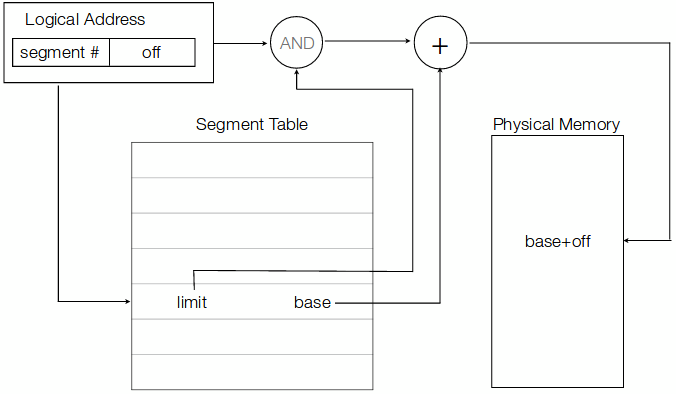
\includegraphics[scale=0.5]{segtab.png}
\end{frame}
\subsection{Mapping}
\begin{frame}
\frametitle{Mapping}
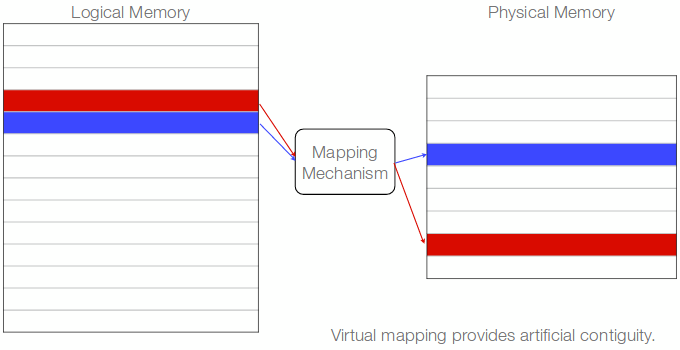
\includegraphics[scale=0.5]{mapping.png}
\end{frame}
%-----------------------------------------------------------------
\section{Paging}
\begin{frame}
\frametitle{Paging}
\begin{itemize}
\item Need to efficiently map between address spaces
\item Cannot map individual locations, would take more memory than is physically available
\item Instead system tracks blocks of memory
\item Virtual memory is divided into pages
\item Physical memory is divided into page frames
\item Typical page sizes range from 512Bytes to 16KB.
\item Each process has a page table:
\begin{itemize}
\item An array of page table entries
\item One entry for each page in memory
\end{itemize}
\item A page table entry is typically a 32-bit word
\item Allows memory to be protected
\item Process can address only pages in page table
\item Switching processes means switching onlypage table address in MMU.
\end{itemize}
\end{frame}
%----------------------------------------------------------------
\subsection{Page Table Entries}
\begin{frame}
\frametitle{Page Table Entries}
\begin{itemize}
\item Elements in the page table entry:
\begin{itemize}
\item \textbf{pFNo:} Page frame number
\item \textbf{pAccess:} Protection information
\item \textbf{pAvail:} Present/Absent flag
\item \textbf{pUsed:} Referenced flag
\item \textbf{pDirty:} Modified flag
\end{itemize}
\item For each memory reference, the bits of a page are tested to ensure access is valid
\item All tests are done in parallel in hardware
\end{itemize}
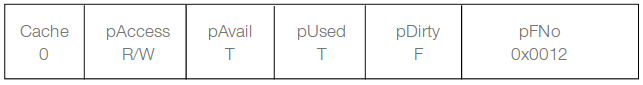
\includegraphics[scale=.35]{pEntry.png}
\end{frame}
%------------------------------------------------------------------
\subsection{MMU registers for Paged Virtual Memory}
\begin{frame}
\frametitle{MMU registers for Paged Virtual Memory}
\begin{itemize}
\item MMU must be able to locate pages in memory
\item For this it uses:
\begin{itemize}
\item \textbf{pTab:} Page table (real) addressfor current process
\item \textbf{pTabSize:} Number of pages in virtual address space
\end{itemize}
\item Demand Paged Virtual Memory:
\end{itemize}
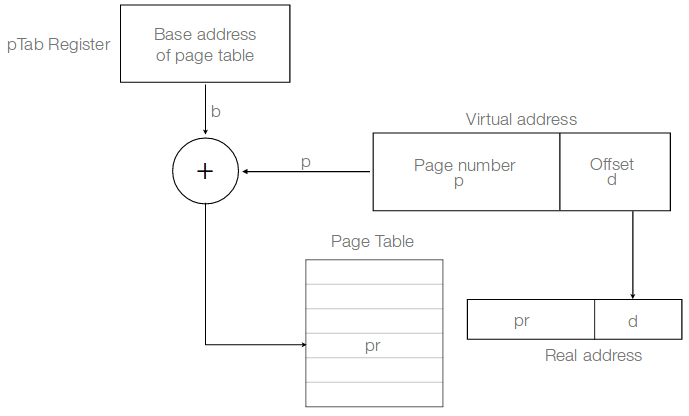
\includegraphics[scale=.3]{deman.png}
\end{frame}
%------------------------------------------------------------------
\subsection{Page Faults}
\begin{frame}
\frametitle{Page Faults}[a;llowpagebreaks]
\begin{itemize}
\item pAvail signifies if a page is available in main memory
\begin{itemize}
\item CPU cannot access secondary memory directly
\item How does it read from page?
\end{itemize}
\item MMU generates a page fault
\item CPU is interrupted and required page is swapped in.
\item Control is transferred to schedular via a trap
\item Faulted process is blocked
\item Control transferred to memory manager
\item DMA used to transfer requested page
\item Memory manager selects a frame to store the page.
\item If no page frames are empty, one must be replaced
\item Possiblepage replacement strategies
\begin{itemize}
\item Least frequently used
\item Least recently used
\item First-in, First-out
\end{itemize}
\item Least frequently used is most favoured
\item MEmory manager checks pDirty bit for old page, if set:
\begin{itemize}
\item Initiate disc transferto save the page
\item Initiate disc transfer to fetch new page
\item Move faulted process to ready queue
\end{itemize}
\end{itemize}
\end{frame}
%-----------------------------------------------------------------
\section{Working Sets}
\begin{frame}
\frametitle{Working Sets}
\begin{itemize}
\item The working set is the active pages over a period of time
\begin{itemize}
\item Usually much less than entire virtual address space
\item Page numbers change gradually over time
\end{itemize}
\item Memory manager imposes a fixed working set size:
\begin{itemize}
\item size is important, to avoid thrashing
\item Excessive disc activity introduces bottlenecks
\end{itemize}
\item Can schedule process only if all working set is available
\end{itemize}
\end{frame}
\subsection{Working Sets Example}
\begin{frame}
\frametitle{Working Sets Example}
\begin{itemize}
\item Suppose:
\begin{itemize}
\item A process has 8 virtual pages
\item Memory manager allocates a working set of 4
\item Page frames in working set are initally empty
\item Memory manager uses least-frequently-used policy
\end{itemize}
\item Assume following sequence of page references:
\begin{itemize}
\item 0,2,4,6,2,1,4,3,2,7,5,3,2,7,6,3,7,2	
\end{itemize}
\end{itemize}
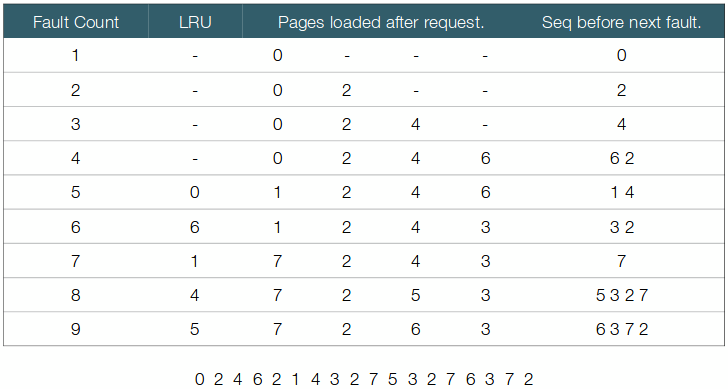
\includegraphics[scale=0.35]{setex.png}
\end{frame}
%----------------------------------------------------------------
\subsection{Pagin and Segmentation}
\begin{frame}
\frametitle{Paging and Segmentation}
\begin{itemize}
\item Fixed block sizes are referred to as pages
\item Variable block sizes are referred to as segments
\begin{itemize}
\item Concept of virtual address being formed of a segment ID and an offset is similar
\end{itemize}
\item Possible to combine both paging and segmentation
\item Also possible to have multi-level page tables
\end{itemize}
\end{frame}
%-------------------------------------------------------------------
\section{Summary}
\begin{frame}
\frametitle{Summary}
\begin{itemize}
\item Programs need to be bound to memory:
\begin{itemize}
\item Some instruction arent complete without address
\item Three situations: compile time, load time, run time
\end{itemize}
\item Memory must be protected and shared
\begin{itemize}
\item MMU enables this
\item Process operates in logical address space
\item MMU translates logical address to physical address.
\end{itemize}
\end{itemize}
\end{frame}
%------------------------------------------------------------------

\begin{frame} 
\Huge{\centerline{The End}}
\end{frame}

\end{document}